\documentclass{article}

%%%%%%%%%%%%%%%%%%%%%%%%%%%%%%%%%%%%%%%%
%% Packages
%%%%%%%%%%%%%%%%%%%%%%%%%%%%%%%%%%%%%%%%

\usepackage[english]{babel}

% Margins
\usepackage[margin=1in]{geometry}
% Spaced paragraphs
\usepackage[parfill]{parskip}
% Fancy headers
\usepackage{fancyhdr}
% Allow use of titles
\usepackage{titling}

% Maths stuff
\usepackage{amsmath}
\usepackage{amsfonts}
\usepackage{amssymb}
\usepackage{amsthm}
\usepackage{physics}
\usepackage{bm}
\usepackage{turnstile}

% Links
\usepackage[hidelinks]{hyperref}

% Allow repetition in macros
\usepackage{multido}

% Set up theorem and definition environments
\newtheorem{theorem}{Theorem}
\newtheorem{definition}{Definition}

%%%%%%%%%%%%%%%%%%%%%%%%%%%%%%%%%%%%%%%%
%% Tikz
%%%%%%%%%%%%%%%%%%%%%%%%%%%%%%%%%%%%%%%%

%\usepackage{subcaption}
\usepackage{tikz}
\usetikzlibrary{automata}
\usetikzlibrary{arrows}
\usetikzlibrary{arrows.meta}
\usetikzlibrary{calc}

\tikzset{
	%	vertex/.style={circle,draw,minimum size=1.5em},
	%	main node/.style={circle,draw,font=\sffamily\Large\bfseries},
	%	main node/.style={circle,thick,draw},
	edge/.style={->,> = latex'}
}

%%%%%%%%%%%%%%%%%%%%%%%%%%%%%%%%%%%%%%%%
%% Set Theory Macros
%%%%%%%%%%%%%%%%%%%%%%%%%%%%%%%%%%%%%%%%

% Naturals
\newcommand{\Nat}{\mathbb{N}}
% Integers
\newcommand{\Int}{\mathbb{Z}}
% Rationals
\newcommand{\Rationals}{\mathbb{Q}}
% Reals
\newcommand{\Reals}{\mathbb{R}}

% Use small arrows for implies / iff
\renewcommand{\implies}{\rightarrow}
\renewcommand{\iff}{\leftrightarrow}

% Use bold for vectors
\renewcommand{\vec}[1]{\mathbf{#1}}

% Notation for a set (easier than \lbrace \rbrace :P)
\newcommand{\set}[1]{\left\lbrace #1 \right\rbrace}

% Notation for a set comprehension / set builder notation
\newcommand{\setcomp}[2]{\set{#1 \, | \, #2}}

% Notation for a set comprehension with two conditions
\newcommand{\setcompdouble}[3]{\set{#1 \, | \, #2 \, | \, #3}}

% Notation for a tuple
\newcommand{\tuple}[1]{\left\langle #1 \right\rangle}

% Notation for a pair
\newcommand{\pair}[2]{\tuple{#1, #2}}

% Powerset
\newcommand{\powerset}[1]{\mathcal{P}(#1)}

% Ordinals
\newcommand{\On}{\bm{On}}
% Language
\newcommand{\Lang}{\mathcal{L}}
% Language of Set Theory
\newcommand{\LangSet}{\Lang_\in}

% Model
\newcommand{\Model}{\mathcal{M}}

% Function notation for injection / surjection / bijection
\newcommand{\surject}{\twoheadrightarrow}
\newcommand{\inject}{\rightarrowtail}
\newcommand{\biject}{\mathbin{\rightarrowtail \hspace{-8pt} \twoheadrightarrow}}

% Russell's set
\newcommand{\RussellSet}{\setcomp{z \in x}{z \notin z}}

%%%%%%%%%%%%%%%%%%%%%%%%%%%%%%%%%%%%%%%%
%% Computability Theory Macros
%%%%%%%%%%%%%%%%%%%%%%%%%%%%%%%%%%%%%%%%

% Turing machine computes
\newcommand{\turingcomputes}[1]{\xrightarrow[#1]{}}

% Projection function
\newcommand{\proj}[2]{\pi_{#1, #2}}

% Proper subtraction / 'monus'
\providecommand{\monus}{% Don't redefine it if available
	\mathbin{% We want a binary operation
		\vphantom{+}% The same height as a plus or minus
		\text{% Change size in sub/superscripts
			\mathsurround=0pt % To be on the safe side
			\ooalign{% Superimpose the two symbols
				\noalign{\kern-.35ex}% but the dot is raised a bit
				\hidewidth$\smash{\cdot}$\hidewidth\cr % Dot
				\noalign{\kern.35ex}% Backup for vertical alignment
				$-$\cr % Minus
			}%
		}%
	}%
}

%%%%%%%%%%%%%%%%%%%%%%%%%%%%%%%%%%%%%%%%
%% Titles
%%%%%%%%%%%%%%%%%%%%%%%%%%%%%%%%%%%%%%%%

\title{MATH3306 Course Notes -- \url{https://github.com/mcoot/CourseNotes} }
\author{Joseph Spearritt}

\pagestyle{fancy}
\lhead{\thetitle}
\rhead{\theauthor}
\cfoot{\thepage}

\begin{document}
	\section{Finite State Automata}

\subsection{Alphabets \& Strings}

\begin{itemize}
	
	\item Let $ A $ be a set; then $ A^n $ is the set of all finite sequences $ a_1 \dots a_n $ with $ a_i \in A $, $ 1 \le i \le m $
	
	\begin{itemize}
		\item Elements of $ A $ are \textit{letters} or \textit{symbols}
		
		\item Elements of $ A^n $ are \textit{words} or \textit{strings} over $ A $ of length $ m $
	\end{itemize}

	\item $ \varepsilon $ is the special \textit{empty string}, the only string of length $ 0 $

	\item $ A^+ = \bigcup_{m \ge 1} A^m $ -- the set of non-empty strings over $ A $ of any length
	
	\item $ A^* = A^+ \cup \varepsilon = \bigcup_{m \ge 0} A^m$ -- the set of (possibly empty) strings over $ A $ of any length
	
	\item If $ \alpha = a_1 \dots a_m $, $ \beta = b_1 \dots b_m \in A^* $, then define $ \alpha \beta $ to be $ a_1 \dots a_m b_1 \dots b_m \in A^{m + n} $. This gives binary `product' or \textit{concatenation} on $ A^* $
	
	\item For $ \alpha \in A^+ $, define $ \alpha^n, n \in \Nat $ by $ \alpha^0 = \varepsilon $, and $ \alpha^{n+1} = \alpha^n \alpha $
	
	\item A \textit{language} with alphabet $ A $ is a subset of $ A^* $
	
\end{itemize}

\clearpage

\subsection{Definition of an FSA}

\begin{itemize}
	
	\item A Finite State Automaton (FSA) is a tuple $ M = (Q, F, A, \tau, q_0) $
	
	\begin{itemize}
		
		\item $ Q $ is a finite set of states
		
		\item $ F \subseteq Q $ is the set of final states
		
		\item $ A $ is the alphabet
		
		\item $ \tau \subseteq Q \times A \times Q $ is the set of transitions
		
		\item $ q_0 \in Q $ is the initial state
		
	\end{itemize}

	\item The transition diagram of an FSA is a directed graph with:
	
	\begin{itemize}
		
		\item Vertex set $ Q $
		
		\item An edge for each transition; $ (q, a, q') \in \tau $ corresponds to an edge from $ q $ to $ q' $ with label $ a $
		
		\item Initial state $ q_0 $ labelled with $ - $
		
		\item Final states labelled with $ + $
		
		\item Example: a \textit{non-deterministic} `haha machine', with $ A = \set{h, a} $
		
		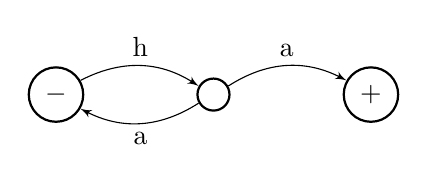
\begin{tikzpicture}
		\node[circle,thick,draw] (q0) at (0, 0) {$ - $};
		\node[circle,thick,draw] (q1) at (2, 0) {$ \; $};
		\node[circle,thick,draw] (q2) at (4, 0) {$ + $};
		
		\draw[edge] (q0) to[bend left] node[above] {h} (q1);
		\draw[edge] (q1) to[bend left] node[above] {a} (q2);
		\draw[edge] (q1) to[bend left] node[below] {a} (q0);
		\end{tikzpicture}
		
	\end{itemize}

	\item A \textit{computation} of $ M $ is a sequence $ q_0, a_1, q_1, a_2, \dots, a_n, q_n $ with $ n \ge 0 $ where $ (q_i, a_{i+1}, q_{i+1}) \in \tau $ for $ 0 \le i \le n - 1 $
	
	\begin{itemize}
		
		\item The \textit{label} on the computation is $ a_1 \dots a_m $
		
		\item The computation is \textit{successful} if $ q_n \in F $
		
		\item A string $ a_1 \dots a_n $ is \textit{accepted} by $ M $ if there is a successful computation with label $ a_1 \dots a_n $, and it is \textit{rejected} otherwise
		
	\end{itemize}

	\item The language recognised by $ M $ is $ \Lang(M) = \setcomp{w \in A^*}{w \text{ is accepted by } M} $
	
	\item There is a one-to-one correspondence between computations of $ M $ and paths in the graph from $ q_0 $	
	
	\item Example: $ A = \set{a, b} $ of an FSA accepting only words with an odd number of 'a's
	
	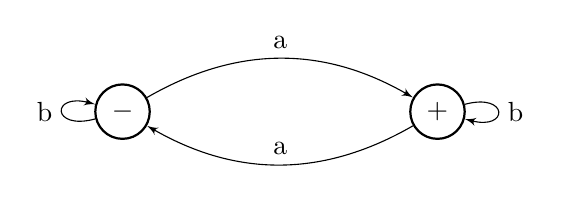
\begin{tikzpicture}
	\node[circle,thick,draw] (q0) at (0, 0) {$ - $};
	\node[circle,thick,draw] (q1) at (4, 0) {$ + $};
	
	\draw[edge] (q0) to[bend left] node[above] {a} (q1);
	\draw[edge] (q0) to[loop left] node[left] {b} (q0);
	
	\draw[edge] (q1) to[bend left] node[above] {a} (q0);
	\draw[edge] (q1) to[loop right] node[right] {b} (q1);
	\end{tikzpicture}
	
	\item An FSA is deterministic (a DFA) if for all $ q \in Q, a \in A $ there is exactly one $ q' \in Q $ such that $ (q, a, q') \in \tau $
	
	\item Example: DFA for the `haha machine'
	
	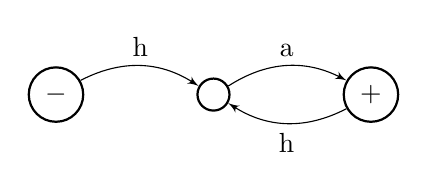
\begin{tikzpicture}
	\node[circle,thick,draw] (q0) at (0, 0) {$ - $};
	\node[circle,thick,draw] (q1) at (2, 0) {$ \; $};
	\node[circle,thick,draw] (q2) at (4, 0) {$ + $};
	
	\draw[edge] (q0) to[bend left] node[above] {h} (q1);
	\draw[edge] (q1) to[bend left] node[above] {a} (q2);
	\draw[edge] (q2) to[bend left] node[below] {h} (q1);
	\end{tikzpicture}
	
	\item Note this machine lacks a transition for $ a $ when in the initial state -- though technically required for a DFA, it is easily fixed by adding an `error state' to catch what would otherwise be missing transitions
	
\end{itemize}

\clearpage

\subsection{Deterministic FSAs}

\begin{itemize}
	
	\item For a DFA $ M $, define the transition function $ \delta: Q \times A \to Q $ by $ q' = \delta(q, a) $, where $ q' $ is the unique element such that $ (q, a, q') \in \tau $
	
	\item If $ \Lang $ is a language with alphabet $ A $, then the following are equivalent:
	
	\begin{enumerate}
		\item $ \Lang $ is recognised by an FSA
		
		\item $ \Lang $ is recognised by a DFA
	\end{enumerate}
	
	\item Given a non-deterministic FSA $ M = (Q, F, A, \tau, q_0) $, an equivalent DFA $ M' = (Q', F', A, \tau', q_0') $ may be generated by the \textit{powerset method}:
	
	\begin{itemize}
		
		\item $ Q' = \powerset{Q} \setminus \emptyset $ (i.e. the set of all subsets of $ Q $ that aren't empty)
		
		\item $ F' = \setcomp{X \in Q'}{q \in X \text{ for some } q \in F} $
		
		\item For $ X \in Q', a \in A $, define $ \delta(X, a) := \setcomp{q \in Q}{(x, a, q) \in \tau \text{ for some } x \in X} $
		
		\item $ \tau' = \setcomp{(X, a, \delta(X, a))}{X \in Q', a \in A} $
		
		\item $ q_0' = \set{q_0} $
		
	\end{itemize}

	\item Proof: show that $ \Lang(M) = \Lang(M') $
	
	\begin{itemize}
		\item $ \Lang(M) \subseteq Lang(M') $:
		
		\begin{itemize}
			\item Given $ w \in \Lang(M) $, $  q_0 a_1 \dots a_n q_n $ is a successful computation of $ M $
			
			\item Then define $ q_i' = \delta(q_{i-1}', a_i) $ for $ 1 \le i \le n $
			
			\item $ q_0', a_1, q_1' \dots a_n, q_n' $ will be a successful computation of $ M' $
			
			\item Therefore $ w \in \Lang(M') $
		\end{itemize}
	
	\item $ \Lang(M') \subseteq Lang(M) $:
	
	\begin{itemize}
		\item Let $ w = a_1 \dots a_n \in L(M') $, and $  q_0', a_1, q_1' \dots a_n, q_n' $ be a successful computation of $ M $
		
		\item Each $ q_i' $ cannot be the empty set
		
		\item By definition of $ \tau' $, $ \exists q_1 \in q_1' $ s.t. $ (q_0, a_1, q_1) \in \tau $
		
		\item Then we can find $ q_i \in q_i' $ s.t. $ (q_{i-1}, a_i, q_i) \in \tau $ for $ 1 \le i \le n $
		
		\item For $ q_n $ we further require $ q_n \in F $
		
		\item Therefore, $ q_0, a_1, q_1, a_2, \dots a_n, q_n $ is a successful computation
		
		\item Therefore $ w \in \Lang(M) $
	\end{itemize}
	
	\end{itemize}
	
\end{itemize}

\clearpage

\subsection{The Pumping Lemma}

\begin{itemize}
	
	\item The Pumping Lemma says that for any $ \Lang $ recognised by an FSA $ M $, there is a certain word length beyond which all words can be split into sections as $ xyz$, where $ x y^n z $ is also in the language
	
	\item Formally there is an integer $ p > 0 $ s.t. any word $ w \in L $ with $ \abs{w} \ge p $ is of the form $ w = xyz $, where $ \abs{y} > 0 $, $ \abs{xy} \le p $ and $ x y^i z \in \Lang $ for $ i \ge 0 $
	
	\item Proof:
	
	\begin{itemize}
		
		\item Let $ p $ be the number of states in $ M $, and suppose $ w = a_1 \dots a_n \in \Lang $, where $ n \ge p $
		
		\item A successful computation $ q_0, a_1, \dots, q_n $ has to pass through a certain state at least twice (by the pigeonhole principle)
		
		\item Therefore, $ \exists r < s $ s.t. $ q_r = q_s $; choose minimal such $ s $
		
		\item Now put $ x = a_1 \dots a_r $, $ y = a_{r+1} \dots a_s $ (note $ \abs{y} > 0$), and $ z = a_{s+1} \dots a_n $
		
		\item By minimality of $ s $, $ q_0, \dots q_{s-1} $ are distinct, and $ \abs{xy} = s \le p $
		
		\item Then, note that $ q_r, a_{r+1}, \dots, q_{s} $ is a loop, which may be validly repeated $ i \ge 0 $ times
		
		\item Therefore, $ x y^i z \in \Lang $
		
	\end{itemize}

	\item Corollary: here exist languages which are not computable by an FSA
	
	\item Example: there is no FSA which can recognise $ \Lang = \setcomp{a^n b^n}{n \in \Nat} $
	
	\item Proof:
	
	\begin{itemize}
		
		\item Assume for a contradiction there exists an FSA $ M $ which can recognise $ \Lang $
		
		\item Let $ p $ be the number from the pumping lemma, and choose $ n \ge p $ and consider $ w = a^n b^n $

		\item By the pumping lemma, $ \exists x, y, z $ s.t. $ a^n b^n = xyz $, with $ \abs{y} \ge 1 $ and $ \abs{xy} \le p \le n $
		
		\item Then $ y $ is written entirely in terms of the letter a, and $ \abs{y} \ge 1 $
		
		\item By the pumping lemma, $ x y^i z \in \Lang $ for all $ i $
		
		\item So choose $ i = 0 $, then some $ w = a^k b^n \in \Lang $ s.t. $ k < n $, which is a contradiction 
		
	\end{itemize}
	
\end{itemize}

	\section{Turing Machines}

\subsection{Definition}

\begin{itemize}
	
	\item A Turing machine is a tuple $ T = (Q, F, A, I, \tau, q_0) $
	
	\begin{itemize}
		
		\item $ Q $ is a finite set of states
		
		\item $ F \subseteq Q $ is the set of final states
		
		\item $ A $ is a finite set, the tape alphabet, with a distinguished blank symbol $ B \in A $
		
		\item $ I $ is a subset of $ A \setminus \set{B} $, the input alphabet
		
		\item $ \tau \subseteq Q \times A \times Q \times A \times \set{L, R} $ is the set of transitions
		
		\item $ q_0 \in Q $ is the initial state
				
	\end{itemize}
	
	\item As in an FSA, non-determinism is allowed
	
	\item The tape is infinite in both directions, but only ever contains a finite number of non-blank symbols
	
	\item A \textit{tape description} for $ T $ is a triple $ (a, \alpha, \beta) $ with $ a \in A $, and $ \alpha: \Nat \to A $ and $ \beta: \Nat \to A $ being functions with $ a(n) = B $ and $ B(n) = B $ for all but finitely many $ n \in \Nat $
	
	\begin{itemize}
		\item So the tape looks like: $ \dots BBB \beta(l) \beta(l - 1) \dots \beta(0) \underline{a} \alpha(0) \alpha(1) \dots \alpha(r) BBB \dots $, with $ l, r \in \Nat $
	\end{itemize}
	
	\item A \textit{configuration} of $ T $ is a tuple $ (q, a, \alpha, \beta) $ where $ q \in Q $ and $ (a, \alpha, \beta) $ is a tape description
	
	\item If $ c = (q, a, \alpha, \beta) $ is a configuration, a configuration $ c' $ is obtained (reachable) from $ c $ by a single move if one of the following holds:
	
	\begin{itemize}
		\item $ (q, a, q', a', L) \in \tau $ and $ c' = (q', \beta(0), \alpha', \beta') $ where:
		$ \alpha'(0) = a', \alpha'(n) = \alpha(n - 1), n > 0 $ and $ \beta'(n) = \beta(n + 1), n \ge 0 $, or
		
		\item $ (q, a, q', a', R) \in \tau $ and $ c' = (q', \alpha(0), \alpha', \beta') $ where:
		$ \alpha'(n) = \alpha(n + 1), n \ge 0 $ and $\beta'(0) = a', \beta'(n) = \beta(n - 1), n > 0 $
	\end{itemize}

	\item A \textit{computation} of $ T $ is a finite sequence of configurations $ c_1, \dots, c_n = c' $ where $ n \ge 1 $ and $ c_{i+1} $ is obtained from $ c_i $ by a single move, for $ 1 \le i \le n - 1 $
	
	\item A configuration is \textit{terminal} if no configuration is reachable from it
	
	\item A computation halts if $ c' $ is terminal (i.e. there is no configuration reachable from $ c' $)
	
	\item We may write $ c \turingcomputes{T} c' $ if there is a computation starting at $ c $ and ending at $ c' $
	
\end{itemize}

\subsection{Turing Machine as Language Recogniser}

\begin{itemize}
	
	\item For $ w = a_1 \dots a_n \in A^* $, let $ c_w = (q_0, \underline{a_1} \dots a_n) $ (recall $ \underline{a_1} \dots a_n $ is a tape description $ (a, \alpha, \beta) $)
	
	\item If $ w = \varepsilon $, we put $ c_w = (q_0, \underline{B}) $
	
	\item The TM $ T $ \textit{accepts} $ w $ if $ c_w \turingcomputes{T} c' $ for some $ c' = (q, 'a', \alpha', \beta') $ with $ q' \in F $
	
	\item The language recognised by $ T $ is $ \Lang(T) = \setcomp{w \in I^*}{w \text{ is accepted by } T } $
	
	\item Note that $ \Lang(T) $ is a language over $ I $ rather than over $ A $
	
	\item $ T $ is deterministic if for every $ (q, a) \in Q \times A $ there is \textit{at most one} element of $ \tau $ starting with $ (q, a) $
	
	\item Then, there is at most one config $ c' $ obtained from $ c $ by a single move; set $ \delta(c) = c' $
	
	\item $ \delta: C \to C $ is then a partial function
	
\end{itemize}

\clearpage

\subsection{Numerical Turing Machines: TMs as Function Calculators}

\begin{itemize}
	
	\item We want to use TMs to describe a partial function $ f: \Nat^n \to \Nat $
	
	\item A \textit{numerical TM} is a deterministic TM $ T = (Q, F, A, I, \tau, q_0) $ with:
	
	\begin{itemize}
		
		\item $ F = I = \emptyset $
		
		\item $ A = \set{0, 1} $, with $ 0 $ as the blank symbol
		
	\end{itemize}

	\item In a numerical TM, the final states $ F $ and input alphabets $ I $ are not relevant
	
	\item For $ \vec{x} = (x_1, \dots, x_n) \in \Nat^n $, define the tape description $ Tape(\vec{x}) = \underline{0} 1^{x_1} 0 1^{x_2} 0 \dots 0 1^{x_n} $
	
	\item Define the partial function $ \varphi_{T, n}: \Nat^n \to \Nat $ as follows:
	
	\begin{itemize}
		
		\item Let $ \vec{x} \in \Nat^n $ be given
		
		\item The initial config of $ T $ is $ (q_0, Tape(\vec{x})) $
		
		\item If $ T $ halts with tape $ \underline{0} 1^{y} = Tape(y) $ for some $ y \in \Nat $, then $ \varphi_{T, n}(\vec{x}) = y $
		
		\item Otherwise, $ \varphi_{T, n} $ is undefined
		
	\end{itemize}

	\item If $ f: \Nat^n \to \Nat = \varphi_{T, n} $ for some numerical TM $ T $, then $ f $ is \textit{TM computable}  
	
	\item Note that when considering TMs as language recognisers, halting is regarded as an error -- but for a numerical TM, it is fine \textit{so long as} it ends with a configuration of the form $ (q, \underline{0}1^y) $ with $ y \in \Nat $
	
	\item Example: an addition function $ S: \Nat^2 \to \Nat $
	
	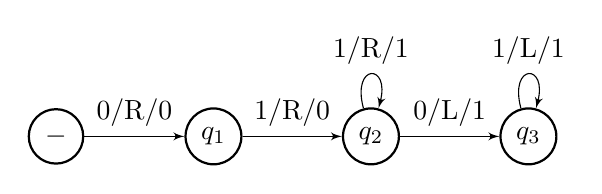
\begin{tikzpicture}
	\node[circle,thick,draw] (q0) at (0, 0) {$ - $};
	\node[circle,thick,draw] (q1) at (2, 0) {$ q_1 $};
	\node[circle,thick,draw] (q2) at (4, 0) {$ q_2 $};
	\node[circle,thick,draw] (q3) at (6, 0) {$ q_3 $};
	
	\draw[edge] (q0) to node[above] {0/R/0} (q1);
	\draw[edge] (q1) to node[above] {1/R/0} (q2);
	\draw[edge] (q2) to node[above] {0/L/1} (q3);
	
	\draw[edge] (q2) to[loop above] node[above] {1/R/1} (q2);
	\draw[edge] (q3) to[loop above] node[above] {1/L/1} (q3);
	\end{tikzpicture}
	
	\item Ultimate theorem: All TM computable functions are partial recursive, and conversely all partial recursive functions are TM computable
	
\end{itemize}

	\section{Partial Recursive Functions}

\subsection{Partial Functions, Definition by Composition \& Primitive Recursion}

\begin{itemize}
	
	\item Classes of functions:
	
	\begin{itemize}
		
		\item Let $ P $ be the set of partial functions, $ P = \setcomp{f}{f \text{ is a partial function } \Nat^n \to \Nat \text{ for some } n > 0} $
		
		\item Let $ T $ be the set of total functions, $ T = \setcomp{f \in P}{f \text{ is total}} $
		
		\item A \textit{class} of functions means a subset of $ P $, and a class of total functions means a subset of $ T $
		
		\item Goal: build a class of functions which we might call `computable'
		
	\end{itemize}
	
	\item Let $ g: \Nat^r \to \Nat, h_1 \dots h_r: \Nat^n \to \Nat $ be partial functions.
	
	Then the partial function $ f: \Nat^n \to \Nat $ obtained from $ g, h_1, \dots, h_r $ by composition is defined by:
	\begin{equation*}
	f(\vec{x}) = g(h_1(\vec{x}), \dots, h_r(\vec{x}))
	\end{equation*}
	\begin{itemize}
		\item We write $f = g \circ (h_1, \dots, h_r) $
	\end{itemize}
	
	\item Let $ g: \Nat^n \to \Nat, h: \Nat^{n+1} \to \Nat $ be partial functions.
	
	Then the partial function $ f: \Nat^{n+1} \to \Nat $ obtained from $ g $ and $ h $ by primitive recursion is defined by:
	\begin{align*}
	&f(\vec{x}, 0) = g(\vec{x})\\
	&f(\vec{x}, y + 1) = h(\vec{x}, y, f(\vec{x}, y))
	\end{align*}
	\begin{itemize}
		\item For a given $ \vec{x} $, $ f(\vec{x}, y) $ is defined for no $ y $, for all $ y $, or for $ 0 \le y \le r $ for some $ r \in \Nat $
		\item Where the `counter' parameter is placed does not matter - it could equally be at the start
	\end{itemize}
	 
\end{itemize}

\subsection{Partial Recursive Functions}

\begin{itemize}
	
	\item We define the \textit{initial functions} to be the following functions:
	
	\begin{itemize}
		
		\item The zero function $ z: \Nat \to \Nat $, such that $ z(x) = 0 $ for all $ x \in \Nat $
		
		\item The successor function $ \sigma: \Nat \to \Nat $, such that $ \sigma(x) = x + 1 $ for all $ x \in \Nat $
		
		\item The projection functions $ \pi_{i, n}: \Nat^n \to \Nat $, where for $ n \ge 1 $ and $ 1 \le i \le n $, $ \pi_{i, n}(x_1, \dots, x_n) = x_i $
		
	\end{itemize}

	\item A class $ \Class $ of total functions is \textit{primitively recursively closed} if:
	
	\begin{itemize}
		
		\item $ \Class $ contains all the initial functions
		
		\item $ \Class $ is closed under composition
		
		\item $ \Class $ is closed under primitive recursion
		
	\end{itemize}

	\item The smallest primitively recursively closed class (i.e. the intersection of all prim. rec. closed classes) is called \textit{the class of primitive recursive functions}
	
	\item Example: addition function $ S: \Nat^2 \to \Nat $, such that $ S(x, y) = x + y $
	\begin{align*}
	S(x, 0) &= g(x), g = \pi_{1, 1}\\
	S(x, y  + 1) &= S(x, y) + 1\\
				 &= \sigma(S(x, y))\\
				 &= h(x, y, S(x, y)), h = \sigma \circ \pi_{3, 3}
	\end{align*}
	
\end{itemize}
	\section{First Order Logic}

\subsection{First Order Languages: Syntax}

\begin{itemize}
	
	\item A \textit{first-order language} (FOL) consists of the following symbols:
	
	\begin{itemize}
		
		\item \textit{Logical symbols} $ \land, \lor, \lnot, \implies, \iff, =, \forall, \exists $ (common to all FOLs)
		
		\item An infinite set of variables, $ x, y, z, \dots $ (also common to all FOLs)
		
		\item Punctuation symbols: parentheses $ ( \text{ and } ) $ and the comma `$ , $' (also common to all FOLs)
		
		\item A (possibly empty) set of constant symbols (e.g. $ 0, 1 $)
		
		\item A (possibly empty) set of function symbols (e.g. $ +, \times, - $)
		
		\item A (possibly empty) set of predicate symbols (e.g. $ < $)
				
	\end{itemize}

	\item Each function and predicate symbol has an associated arity $ n $
	
	\item Only the \textit{non-logical symbols} are specific to the particular language
	
	\item A FOL may be specified by giving only the constant, relation and function symbols
	
	\begin{itemize}
		\item E.g. the first-order language of arithmetic $ \Lang_A $ consists of the following:
		
		\begin{itemize}
			\item The constant symbol $ 0 $
			\item Unary function symbol $ S $ (the successor function)
			\item Two binary function symbols $ + $ and $ \cdot $
		\end{itemize}
	\end{itemize}
	
	\item Given an FOL $ \Lang $, an \textit{expression} of $ \Lang $ is a finite sequence of symbols; not all expressions are \textit{formulae}
	
	\item A \textit{term} of an FOL is defined inductively:
	
	\begin{itemize}
		
		\item Every constant symbol in $ \Lang $ is a term
		
		\item Every variable symbol in $ \Lang $ is a term
		
		\item If $ t_1, \dots, t_n $ are terms and $ f $ is an $ n $-ary function symbol in $ \Lang $, then $ f(t_1, \dots t_n) $ is a term in $ \Lang $
		
	\end{itemize}

	\item An \textit{atomic formula} of an FOL is defined as follows:
	
	\begin{itemize}
		\item If $ t_1 $ and $ t_2 $ are terms, then $ t_1 = t_2 $ is an atomic formula
		
		\item If $ F $ is an $ n $-ary predicate and $ t_1, \dots, t_n $ are terms, then $ F(t_1, \dots, t_n) $ is an atomic formula
	\end{itemize}

	\item A \textit{formula} of an FOL is defined inductively:
	
	\begin{itemize}
		
		\item An atomic formula is a formula
		
		\item If $ \phi $ and $ \psi $ are both formulae, then so are $ \lnot \phi $, $ \phi \land \psi $, $ \phi \lor \psi $, $ \phi \implies \psi $, and $ \phi \iff \psi $
		
		\item If $ \phi $ is a formula and $ x $ is a variable symbol, then $ \exists x \phi $ and $ \forall x \phi $ are formulae
		
		\item Parentheses should be used as necessary to ensure there is exactly one way of reading a formula
		
	\end{itemize}

	\item A variable is \textit{bound} by a quantifier $ \forall x $ or $ \exists x $ in a formula $ \phi $ if:
	
	\begin{itemize}
		\item $ x $ is in the scope of the quantifier; and
		
		\item the scope of the quantifier contains no other quantifiers over $ x $ with $ x $ in their scope
	\end{itemize}

	\item Any variable which is not bound in a formula $ \phi $ is \textit{free} in $ \phi $
	
	\item A \textit{sentence} of an FOL is a formula with no free variables
	
	\item Importantly, an FOL gives no \textit{meaning} to formulae -- they are not `true' or `false'
		
\end{itemize}

\subsection{Models: Semantics}

\begin{itemize}
	
	\item For an FOL $ \Lang $, an \textit{$ \Lang $-structure} or \textit{model} $ \Model $ consists of the following:
	
	\begin{itemize}
		\item A domain or universe: a non-empty set $ \abs{\Model} $
		
		\item Interpretation for constant symbols: for each constant symbol $ c $ of $ \Lang $, an element $ c^\Model \in \abs{\Model} $
		
		\item Interpretation for predicate symbols: for each $ n $-ary predicate symbol $ R $ of $ \Lang $, an $ n $-ary predicate $ R^\Model \subseteq \abs{\Model}^n $
		
		\item Interpretation for function symbols: for each $ n $-ary function symbol $ f $ of $ \Lang $, an $ n $-ary function $ f^\Model: \abs{\Model}^n \to \abs{\Model} $
	\end{itemize}

	\item A sentence of $ \Lang $ acquires \textit{meaning} when an $ \Lang $-structure $ \Model $ is given and the sentence is interpreted within $ \Model $
	
	\item We can determine the truth value of a formula $ \phi $ (possibly with free variables) in $ \Lang $-structure $ \Model $ if a \textit{variable assignment} $ \alpha: \text{ set of variable symbols} \to \abs{\Model} $ is given
	
	\item For given $ \alpha $, replace all free variables $ x_i $ in $ \phi $ by $ \alpha(x_i) $, so $ \phi $ becomes a statement in $ \Model $ which must either be true or false
	
	\item We say a formula $ \phi $ is \textit{true in $ \Model $} if $ \phi $ is true for \textbf{any} variable assignment $ \alpha $
	
	\item For a sentence $ \phi $ in $ \Lang $, its truth values does not depend on variable assignment (since there is no free variable). Thus $ \phi $ must be either true or false in $ \Model $, independent of variable assignment
	
\end{itemize}

\newpage

\subsection{Axiomatic Systems \& Proof}

\begin{itemize}
	
	\item A formal axiomatic system comprises:
	
	\begin{itemize}
		
		\item A first-order language
		
		\item Syntactic rules for constructing formulae from the symbols
		
		\item A collection of axioms
		
		\item Rules of inference
		
	\end{itemize}

	\item From the axioms we obtain other formulae using the rules of inference, called \textit{theorems}
	
	\item A \textit{proof} of a theorem is the process of applying the rules
	
	\item A set of \textit{Logical axioms} are common to first-order axiomatic systems
	
	\item We may also state theory-specific \textit{non-logical axioms}
	
	\item Two logical inference rules are also provided:
	
	\begin{itemize}
		\item Modus ponens: $ \prftree[r]{}{\phi \implies \psi, \phi}{\psi} $
		
		\item Generalisation: $ \prftree[r]{}{\phi}{\forall x \phi} $
	\end{itemize}
	
	\item Given $ T $, a `theory' or (possibly empty) set of non-logical axioms in $ \Lang $, a formula $ \psi $ is \textit{provable} in $ T $, denoted $ T \vdash \psi $ if there is a finite sequence $ \phi_1, \dots, \phi_n $ of formulae such that $ \phi_n $ is equal to $ \psi $ and for all $ i $ with $ 1 \le i \le n $ we have:
	
	\begin{itemize}
		
		\item $ \phi_i $ is a logical axiom; or
		
		\item $ \phi_i \in T $; or
		
		\item There are $ j, k < i $ such that $ \phi_j $ is equal to the formula $ \phi_k \implies \phi_i $; or
		
		\item There is a $ j < i $ such that $ \phi_i $ is equal to the formula $ \forall x \phi_j $
		
	\end{itemize}

	\item If a formula $ \psi $ is not provable in $ T $, then we write $ T \nvdash \psi $
	
	\item A formula $ \phi $ is a \textit{tautology} if $ \vdash \phi $ (i.e. it may be proved with no theory-specific axioms)
	
	\item We say two formulae $ \phi $ and $ \psi $ are \textit{equivalent}, denoted $ \phi \equiv \psi $ if $ \vdash \phi \iff \psi $; that is, if $ \phi \iff \psi $ is a tautology
	
	\item We say a theory $ T $ is \textit{consistent} if there is no formula $ \phi $ in $ \Lang $ such that $ T \vdash (\phi \land \lnot \phi) $
	
	\begin{itemize}
		\item If $ T $ is inconsistent, then for all formulae $ \psi $ in $ \Lang $ we have $ T \vdash \psi $
		
		\subitem \textit{``From contradiction, everything follows"}
	\end{itemize}

	\item We say a theory $ T $ is \textit{complete} if for all formulae $ \phi $ in $ \Lang $, $ T \vdash \phi $ or $ T \vdash \lnot \phi $	
	
\end{itemize}
\end{document}